%% Preamble 
\documentclass[11pt,a4paper]{article}
\usepackage[utf8]{inputenc}
\usepackage[T1]{fontenc}
\usepackage{lmodern}
\usepackage[margin=25mm]{geometry}
\usepackage{amsmath,amssymb,mathtools,bm,array,xcolor,booktabs,longtable}
\usepackage{tikz,microtype,enumitem}
\usepackage[nolist]{acronym}
\usetikzlibrary{arrows.meta,positioning,fit}
\usepackage[colorlinks=true,linkcolor=blue!50!black,urlcolor=blue!50!black]{hyperref}
\newenvironment{example}[1]{\par\medskip\noindent\textbf{Worked example: #1.}\ }{\par\medskip}
\setlist[itemize]{noitemsep}
\numberwithin{equation}{section}
\setcounter{tocdepth}{1}

%%%%%%%%%%%%%%%%%%%%%%%%%%%%%%%%%%%%%%%%%%%%%%%%%%%%%%%%%%%%
% MIMO Communications - Common LaTeX Commands
%%%%%%%%%%%%%%%%%%%%%%%%%%%%%%%%%%%%%%%%%%%%%%%%%%%%%%%%%%%%
% Required packages:
% \usepackage{amsmath,amssymb,amsfonts}
% \usepackage{mathtools}
% \usepackage{bm}
% \usepackage{array}
% \usepackage{xcolor}
%
% Convention:
% - Scalars: italic
% - Vectors/matrices: bold lowercase/uppercase
% - Sets: calligraphic
% - Descriptive indices: \mathsf
% - Matrix transpose markers: \mathsf
% - Named mathematical operators: upright
%%%%%%%%%%%%%%%%%%%%%%%%%%%%%%%%%%%%%%%%%%%%%%%%%%%%%%%%%%%%


%%%%%%%%%%%%%%%%%%%%%%%%%%%%%%%%%%%%%%%%%%%%%%%%%%%%%%%%%%%%
% 1. REVIEW AND EDITING
%%%%%%%%%%%%%%%%%%%%%%%%%%%%%%%%%%%%%%%%%%%%%%%%%%%%%%%%%%%%

% Display old text [blue] and proposed text [red]
\newcommand{\Review}[2]{%
	{\color{blue}[#1]}{\color{red}[#2]}}

% Display corrected versions
\newcommand{\Fixed}[2]{%
	{\color{orange}[#1]}{\color{green}[#2]}}

% Show only the accepted version (first argument)
\newcommand{\Done}[2]{#1}

% Comments and notes
\newcommand{\Response}[1]{{\color{magenta}[#1]}}
\newcommand{\Note}[1]{{\color{blue}[#1]}}


%%%%%%%%%%%%%%%%%%%%%%%%%%%%%%%%%%%%%%%%%%%%%%%%%%%%%%%%%%%%
% 2. GENERAL UTILITIES
%%%%%%%%%%%%%%%%%%%%%%%%%%%%%%%%%%%%%%%%%%%%%%%%%%%%%%%%%%%%

% Fixed-width table columns with proper line breaks
\newcolumntype{C}[1]{>{\centering\arraybackslash}p{#1}}
\newcolumntype{R}[1]{>{\raggedleft\arraybackslash}p{#1}}
\newcolumntype{L}[1]{>{\raggedright\arraybackslash}p{#1}}

% Display literal LaTeX text
\newcommand{\ttplain}[1]{\texttt{\detokenize{#1}}}

% Underbraces for expressions in matrices/arrays
\newcommand{\undermat}[2]{%
	\makebox[0pt][l]{$%
		\smash{%
			\underbrace{%
				\phantom{\begin{matrix}#2\end{matrix}}%
			}_{\text{$#1$}}%
		}$}#2}

\newcommand{\coolunder}[2]{%
	\mathrlap{%
		\smash{%
			\underbrace{%
				\phantom{\begin{matrix}#2\end{matrix}}%
			}_{\mbox{$#1$}}%
		}%
	}#2}


%%%%%%%%%%%%%%%%%%%%%%%%%%%%%%%%%%%%%%%%%%%%%%%%%%%%%%%%%%%%
% 3. CROSS-REFERENCING
%%%%%%%%%%%%%%%%%%%%%%%%%%%%%%%%%%%%%%%%%%%%%%%%%%%%%%%%%%%%

\newcommand{\figref}[1]{Figure.~\ref{#1}}
\newcommand{\secref}[1]{Section~\ref{#1}}
\newcommand{\chapref}[1]{Chapter~\ref{#1}}
\newcommand{\theref}[1]{Theorem~\ref{#1}}
\newcommand{\appref}[1]{Appendix~\ref{#1}}
\newcommand{\tabref}[1]{Table~\ref{#1}}

% Define if not already provided by another package
\providecommand{\algref}[1]{}
\renewcommand{\algref}[1]{Algorithm~\ref{#1}}
% Additional packages for notation tables
\usepackage{longtable}
\usepackage{array}
%% MATH NOTATION
%%%%%%%%%%%%%%%%%%%%%%%%%%%%%%%%%%%%%%%%%%%%%%%%%%%%%%%%%%%%
% 4. MATHEMATICAL OPERATORS AND DELIMITERS
%%%%%%%%%%%%%%%%%%%%%%%%%%%%%%%%%%%%%%%%%%%%%%%%%%%%%%%%%%%%

% Ceiling and floor (mathtools)
\DeclarePairedDelimiter{\ceil}{\lceil}{\rceil}
\DeclarePairedDelimiter{\floor}{\lfloor}{\rfloor}

% Optimization operators
\DeclareMathOperator*{\argmax}{arg\,max}
\DeclareMathOperator*{\argmin}{arg\,min}
\DeclareMathOperator*{\argfirst}{arg\,first}

% Angle/phase of complex quantity
% Overrides any existing \ang definition
\providecommand{\ang}[1]{}
\renewcommand{\ang}[1]{%
	\operatorname{angle}\left(#1\right)}

% Definition symbol
\newcommand{\define}{\triangleq}

% Delimiters (legacy commands)
\newcommand{\LeftP}{\left\lbrace}
\newcommand{\RightP}{\right\rbrace}
\newcommand{\LeftPD}{\left(}
\newcommand{\RightPD}{\right)}

% Additional delimiters
\newcommand{\Abs}[1]{\left|#1\right|}
\newcommand{\inner}[2]{%
	\left\langle #1,#2\right\rangle}


%%%%%%%%%%%%%%%%%%%%%%%%%%%%%%%%%%%%%%%%%%%%%%%%%%%%%%%%%%%%
% 5. SETS AND NUMBER FIELDS
%%%%%%%%%%%%%%%%%%%%%%%%%%%%%%%%%%%%%%%%%%%%%%%%%%%%%%%%%%%%

\newcommand{\compl}{\mathbb{C}}   % Complex field
\newcommand{\real}{\mathbb{R}}    % Real field
\newcommand{\intg}{\mathbb{Z}}    % Integers
\newcommand{\galois}{\mathbb{F}_2} % Binary finite field

% Calligraphic sets
\newcommand{\set}[1]{\mathcal{#1}}


%%%%%%%%%%%%%%%%%%%%%%%%%%%%%%%%%%%%%%%%%%%%%%%%%%%%%%%%%%%%
% 6. VECTORS AND MATRICES
%%%%%%%%%%%%%%%%%%%%%%%%%%%%%%%%%%%%%%%%%%%%%%%%%%%%%%%%%%%%

% Bold lowercase vectors and uppercase matrices
\newcommand{\ma}[1]{\bm{#1}}

% Element indexing
\newcommand{\IndexM}[3]{#1\left[#2,#3\right]}
\newcommand{\IndexV}[2]{#1\left[#2\right]}

% Norms
\newcommand{\Norm}[1]{\left\|#1\right\|}
\newcommand{\NormTwo}[1]{\left\|#1\right\|_2}
\newcommand{\frob}[1]{\left\|#1\right\|_{\mathsf{F}}}

% Matrix operations
\newcommand{\inv}[1]{{#1}^{-1}}
\newcommand{\pinv}[1]{{#1}^{+}}        % Pseudoinverse
\newcommand{\mT}[1]{{#1}^{\mathsf{T}}} % Transpose
\newcommand{\mH}[1]{{#1}^{\mathsf{H}}} % Hermitian transpose
\newcommand{\mC}[1]{{#1}^{*}}         % Complex conjugate

% Matrix properties and functions
\newcommand{\trace}[1]{%
	\operatorname{tr}\left(#1\right)}
\newcommand{\rank}[1]{%
	\operatorname{rank}\left(#1\right)}
\newcommand{\Cond}[1]{%
	\operatorname{cond}\left(#1\right)}
\newcommand{\Det}[1]{%
	\operatorname{det}\left(#1\right)}
\newcommand{\diag}[1]{%
	\operatorname{diag}\left(#1\right)}

% Alias for compatibility
\newcommand{\diagM}[1]{\diag{#1}}

% Vector subspaces
\newcommand{\Span}[1]{%
	\operatorname{span}\left(#1\right)}
\newcommand{\Null}[1]{%
	\operatorname{null}\left(#1\right)}
\newcommand{\Range}[1]{%
	\operatorname{range}\left(#1\right)}

% Vectorization and reshaping
\newcommand{\Vect}[1]{%
	\operatorname{vec}\left(#1\right)}
\newcommand{\unvec}[3]{%
	\operatorname{unvec}_{#2\times #3}\left(#1\right)}

% Matrix products
\newcommand{\elemProd}[2]{#1\odot #2}
\newcommand{\elemDiv}[2]{#1\oslash #2}
\newcommand{\kronProd}[2]{#1\otimes #2}


%%%%%%%%%%%%%%%%%%%%%%%%%%%%%%%%%%%%%%%%%%%%%%%%%%%%%%%%%%%%
% 7. PROBABILITY AND STATISTICS
%%%%%%%%%%%%%%%%%%%%%%%%%%%%%%%%%%%%%%%%%%%%%%%%%%%%%%%%%%%%

% Expectation and variance
\newcommand{\Ex}[1]{%
	\mathbb{E}\left[#1\right]}
\newcommand{\Var}[1]{%
	\operatorname{Var}\left[#1\right]}

% Covariance and correlation
\newcommand{\Cov}[2]{%
	\operatorname{Cov}\left(#1,#2\right)}
\newcommand{\Corr}[2]{%
	\operatorname{Corr}\left(#1,#2\right)}

% Probability of an event
\newcommand{\Prob}[1]{%
	\Pr\left(#1\right)}

% Mean-square error
\newcommand{\MSE}[1]{%
	\operatorname{MSE}\left(#1\right)}

% Distribution notation
\newcommand{\Normal}{\mathcal{N}}
\newcommand{\CNormal}{\mathcal{CN}}

% Complex signal operations
\newcommand{\RE}[1]{%
	\operatorname{Re}\left\{#1\right\}}
\newcommand{\IM}[1]{%
	\operatorname{Im}\left\{#1\right\}}


%%%%%%%%%%%%%%%%%%%%%%%%%%%%%%%%%%%%%%%%%%%%%%%%%%%%%%%%%%%%
% 8. SIGNAL PROCESSING OPERATIONS
%%%%%%%%%%%%%%%%%%%%%%%%%%%%%%%%%%%%%%%%%%%%%%%%%%%%%%%%%%%%

% Fourier transform
\newcommand{\FT}[1]{%
	\mathcal{F}\left\{#1\right\}}

% Circular convolution
\newcommand{\circConv}[2]{#1\circledast #2}

% Modulo reduction notation
\newcommand{\modulo}[2]{%
	\left\langle #1\right\rangle_{#2}}

% Sinc function
\newcommand{\Sinc}[1]{%
	\operatorname{sinc}\left(#1\right)}


%%%%%%%%%%%%%%%%%%%%%%%%%%%%%%%%%%%%%%%%%%%%%%%%%%%%%%%%%%%%
% 9. MIMO DIMENSIONS AND INDICES
%%%%%%%%%%%%%%%%%%%%%%%%%%%%%%%%%%%%%%%%%%%%%%%%%%%%%%%%%%%%

% Subscripts t/r: transmit/receive interfaces
% Superscripts rf/a: RF-chain/antenna-element interfaces
% No superscript: effective digital signal ports
% S: number of data streams
%
% Descriptive indices are upright (\mathsf).
% Running mathematical indices are italic..

% Digital signal ports
\newcommand{\NT}{N_{\mathsf{t}}}
\newcommand{\NR}{N_{\mathsf{r}}}
\newcommand{\nT}{n_{\mathsf{t}}}
\newcommand{\nR}{n_{\mathsf{r}}}

% Data streams
\newcommand{\NS}{S}
\newcommand{\nS}{s}

% RF chains
\newcommand{\NTrf}{N_{\mathsf{t}}^{\mathsf{rf}}}
\newcommand{\NRrf}{N_{\mathsf{r}}^{\mathsf{rf}}}
\newcommand{\nTrf}{n_{\mathsf{t}}^{\mathsf{rf}}}
\newcommand{\nRrf}{n_{\mathsf{r}}^{\mathsf{rf}}}

% Physical antenna elements
\newcommand{\NTa}{N_{\mathsf{t}}^{\mathsf{a}}}
\newcommand{\NRa}{N_{\mathsf{r}}^{\mathsf{a}}}
\newcommand{\nTa}{n_{\mathsf{t}}^{\mathsf{a}}}
\newcommand{\nRa}{n_{\mathsf{r}}^{\mathsf{a}}}


%%%%%%%%%%%%%%%%%%%%%%%%%%%%%%%%%%%%%%%%%%%%%%%%%%%%%%%%%%%%
% 10. MIMO PRECODING AND COMBINING MATRICES
%%%%%%%%%%%%%%%%%%%%%%%%%%%%%%%%%%%%%%%%%%%%%%%%%%%%%%%%%%%%

% Digital precoding and combining
\newcommand{\FD}{\ma{F}_{\mathsf{D}}}
\newcommand{\WD}{\ma{W}_{\mathsf{D}}}

% Analog precoding and combining
\newcommand{\FA}{\ma{F}_{\mathsf{A}}}
\newcommand{\WA}{\ma{W}_{\mathsf{A}}}


% MIMO channel representations

\newcommand{\Ha}{\ma{H}_{\mathsf{a}}}
% Antenna-level channel (physical antenna elements)

\newcommand{\Hrf}{\ma{H}_{\mathsf{rf}}}
% Effective channel after analog TX/RX processing


% H_a: Physical antenna-to-antenna channel
% H_rf: Effective channel between RF-chain interfaces
% H: Effective channel between digital signal ports
% H_s: Effective channel between data streams
%
% H_rf = W_A^H H_a F_A
% H    = W_D^H H_rf F_D
% H_s  = W^H H F


\newcommand{\Hs}{\ma{H}_{\mathsf{s}}}
% Effective stream-level channel after digital
% precoding and combining

% Diversity and multiplexing performance
\providecommand{\odiv}{o_{\mathsf{div}}}   % Diversity order
\providecommand{\gmux}{g_{\mathsf{mux}}}   % Multiplexing gain


%%%%%%%%%%%%%%%%%%%%%%%%%%%%%%%%%%%%%%%%%%%%%%%%%%%%%%%%%%%%
% 11. SIGNAL ENERGY AND NOISE
%%%%%%%%%%%%%%%%%%%%%%%%%%%%%%%%%%%%%%%%%%%%%%%%%%%%%%%%%%%%

\newcommand{\Es}{E_{\mathsf{s}}} % Energy per symbol
\newcommand{\Ed}{E_{\mathsf{d}}} % Total energy

\newcommand{\Eb}{E_{\mathsf{b}}} % Energy per bit

% Noise power spectral density parameter
\newcommand{\Nzero}{N_{0}}

\newcommand{\Ptx}{P_{\mathsf{t}}}
\newcommand{\Prx}{P_{\mathsf{r}}}


%%%%%%%%%%%%%%%%%%%%%%%%%%%%%%%%%%%%%%%%%%%%%%%%%%%%%%%%%%%%
% 12. COMMUNICATION METRICS AND ALGORITHMS
%%%%%%%%%%%%%%%%%%%%%%%%%%%%%%%%%%%%%%%%%%%%%%%%%%%%%%%%%%%%

\newcommand{\SNR}{\mathsf{SNR}}
\newcommand{\SINR}{\mathsf{SINR}}
\newcommand{\CSI}{\mathsf{CSI}}

% Combining and precoding
\newcommand{\MRT}{\mathsf{MRT}}
\newcommand{\MRC}{\mathsf{MRC}}
\newcommand{\ZF}{\mathsf{ZF}}
\newcommand{\LMMSE}{\mathsf{LMMSE}}

% Additional commonly used methods
\newcommand{\LS}{\mathsf{LS}}
\newcommand{\MMSE}{\mathsf{MMSE}}
\newcommand{\ML}{\mathsf{ML}}
\newcommand{\MAP}{\mathsf{MAP}}
\newcommand{\RZF}{\mathsf{RZF}}





%%%%%%%%%%%%%%%%%%%%%%%%%%%%%%%%%%%%%%%%%%%%%%%%%%%%%%%%%%%%
% End of common notation
%%%%%%%%%%%%%%%%%%%%%%%%%%%%%%%%%%%%%%%%%%%%%%%%%%%%%%%%%%%%
%% Acronyms
\begin{acronym}
	\acro{p2p}[P2P]{point-to-point}
	\acro{mimo}[MIMO]{multiple-input multiple-output}
	\acro{siso}[SISO]{single-input single-output}
	\acro{simo}[SIMO]{single-input multiple-output}
	\acro{miso}[MISO]{multiple-input single-output}
	\acro{mrc}[MRC]{maximum ratio combining}
	\acro{mrt}[MRT]{maximum ratio transmission}
	\acro{zf}[ZF]{zero forcing}
	\acro{lmmse}[LMMSE]{linear minimum mean-square error}
	\acro{mmse}[MMSE]{minimum mean-square error}
	\acro{svd}[SVD]{singular value decomposition}
	\acro{evd}[EVD]{eigenvalue decomposition}
	\acro{snr}[SNR]{signal-to-noise ratio}
	\acro{sinr}[SINR]{signal-to-interference-plus-noise ratio}
	\acro{csi}[CSI]{channel state information}
	\acro{csir}[CSIR]{channel state information at the receiver}
	\acro{csit}[CSIT]{channel state information at the transmitter}
	\acro{rf}[RF]{radio frequency}
	\acro{qpsk}[QPSK]{quadrature phase-shift keying}
	\acro{awgn}[AWGN]{additive white Gaussian noise}
	\acro{psd}[PSD]{power spectral density}
	\acro{map}[MAP]{maximum a posteriori}
	\acro{mse}[MSE]{mean squared error}
	\acro{ls}[LS]{least squares}
	\acro{ml}[ML]{maximum likelihood }
	\acro{bpsk}[BPSK]{binary phase-shift keying}
	\acro{iid}[IID]{independent and identically distributed}
	\acro{los}[LOS]{line of sight}
	\acro{ostbc}[OSTBC]{orthogonal space-time block code}
	\acro{stbc}[STBC]{space-time block code}
	\acro{dmt}[DMT]{diversity--multiplexing tradeoff}
	\acro{pdf}[PDF]{probability density function}
	\acro{mumimo}[MU-MIMO]{multiuser multiple-input multiple-output}
	\acro{ul}[UL]{uplink}
	\acro{dl}[DL]{downlink}
	\acro{fdma}[FDMA]{frequency-division multiple access}
	\acro{tdma}[TDMA]{time-division multiple access}
	\acro{sdma}[SDMA]{space-division multiple access}
	\acro{bs}[BS]{base station}
	\acro{mac}[MAC]{multiple-access channel}
	\acro{bc}[BC]{broadcast channel}
	\acro{rzf}[RZF]{regularized zero forcing}
	\acro{sic}[SIC]{successive interference cancellation}
	\acro{dpc}[DPC]{dirty-paper coding}
	\acro{dof}[DoF]{degrees of freedom}
	\acro{tdd}[TDD]{time-division duplex}
	\acro{fdd}[FDD]{frequency-division duplex}
	\acro{ap}[AP]{access point}
	\acro{cpu}[CPU]{central processing unit}
	\acro{comp}[CoMP]{coordinated multipoint}
	\acro{cscg}[CSCG]{circularly symmetric complex Gaussian}
	\acro{mu}[MU]{multi-user}
	\acro{se}[SE]{spectral efficiency}
\end{acronym}


%% Title
\title{MIMO Communications\\Lecture 01: Introduction and Mathematical Foundations}
\author{Ahmad Nimr}
\date{Winter Semester 2026/27}

\begin{document}
\maketitle
\begin{abstract}
Multiple antennas provide spatial resources for improving signal quality, reliability, and spectral efficiency. This chapter presents the narrowband digital model from a familiar communication chain, explains the role of channel rank, and distinguishes antenna ports from independent data streams. The appendices introduce the mathematical background needed throughout the course: complex linear algebra, \ac{svd}, \ac{evd}, pseudoinverses, covariance, complex Gaussian vectors, estimation, and detection. Worked examples and a tutorial connect these tools to communication problems.
\end{abstract}
\tableofcontents
\acresetall
\newpage
\section{Learning path}
The lecture addresses three questions about \ac{mimo} systems: 
\emph{Why MIMO? What is MIMO? How is MIMO  modeled?} The course requires basic familiarity with digital modulation, sampling, and elementary matrix multiplication. Students should be able to identify \ac{siso}, \ac{simo}, \ac{miso}, and \ac{mimo} configurations; distinguish array gain, diversity, and spatial multiplexing; formulate a dimensionally consistent digital model; and explain why antenna count alone does not determine the number of useful streams. The teaching narrative follows three steps: why additional antennas are beneficial, what spatial resources they provide, and how processing exploits these resources.

%The first meeting follows the conceptual path in the draft. Detailed mathematical derivations are supporting material, rather than additional topics that must all fit into 90 minutes. Appendices~\ref{app:algebra} and~\ref{app:probability} can be read before Lecture~02 and revisited as needed.
%\begin{center}
%\begin{tabular}{lr}\toprule
%Teaching block & Minutes\\\midrule
%Motivation and MIMO benefits & 15\\
%Communication chain and signal representations & 10\\
%SISO, SIMO, MISO, and MIMO & 20\\
%Rank and spatial dimensions & 15\\
%Digital model, processing, and mathematical previews & 25\\
%Summary and course roadmap & 5\\\midrule
%Total & 90\\\bottomrule
%\end{tabular}
%\end{center}

\section{Why multiple antennas?}


\subsection{Performance objectives and resource limits}
\label{sec:performance_objectives}

The fundamental objective of a communication system is to transfer
information from a source to a destination reliably and efficiently.
The achievable performance depends on the available resources, the
characteristics of the communication channel, and the techniques
used to transmit and recover information. Before introducing the
mathematical model,  a simple physical analogy is considered to
illustrate the potential benefits of multiple transmission paths.

\subsubsection*{A water-pipe analogy}

Consider a system that transfers water from a source to a destination
through a single pipe, driven by a pump. The objective is to deliver
as much water as possible per unit time. The achievable flow is
limited by  cross-sectional area of the pipe, the available pumping
power, and losses caused by friction, leakage, or obstructions.
Additional disturbances may affect the delivery process, while
a complete pipe failure can interrupt the flow.

Several possibilities exist for improving the system:
\begin{itemize}
	\item \textbf{Increase the pipe cross-section:}
	A wider pipe can accommodate greater water flow under suitable
	operating conditions.
	
	\item \textbf{Increase the pumping power:}
	Additional energy can overcome flow resistance and increase
	the delivered amount.
	
	\item \textbf{Improve the pipe characteristics:}
	Reducing friction, leakage, and obstructions makes the
	transfer more efficient.
\end{itemize}
%
However, these improvements require additional resources and may
become increasingly costly. Furthermore, relying on a single pipe
introduces a potential point of failure.

\vspace{10pt}
An alternative is to introduce multiple pipes or branches.
Depending on their arrangement, they can provide different benefits:

\begin{enumerate}
	\item \textbf{Parallel transfer:}
	Several independent pipes can simultaneously transport water,
	potentially increasing the total delivered amount. The flow
	may be directed to a single destination or distributed among
	several destinations.
	
	\item \textbf{Redundant delivery:}
	A single flow can be distributed across multiple branches
	and collected again at the destination. If one branch is
	obstructed or damaged, the remaining branches may continue
	delivering water, improving reliability.
	
	\item \textbf{Combining resources:}
	Multiple sources or pumps can feed a common delivery path,
	increasing the amount of water that can be collected or
	supplied. The improvement depends on the available resources
	and how effectively they are combined.
	
	\item \textbf{Interconnected networks:}
	Multiple sources, branches, and destinations can form a
	network supporting different objectives, including increased
	throughput, reliability, resource sharing, and simultaneous
	service to multiple destinations.
\end{enumerate}
%
These examples illustrate a general principle:
introducing multiple paths provides additional flexibility in
how resources are used, how material is transported, and how
failures are handled.

\vspace{10pt}
Similar opportunities arise in wireless communication through
the use of multiple antennas. Depending on the channel and the
adopted transmission strategy, multiple antennas can improve
received signal quality (\emph{array gain}), provide robustness
against channel variations (\emph{diversity gain}), or support
the simultaneous transmission of independent data streams
(\emph{spatial multiplexing}). Multiple antennas can also serve
different users through spatially selective transmission and
reception.

\paragraph*{Note:} This analogy is conceptual rather than mathematical. Water flow
is governed by fluid mechanics, whereas wireless communication
relies on electromagnetic wave propagation and the transmission
of information through noisy channels. In particular,
electromagnetic signals combine according to their complex
amplitudes and phases, and multiple antennas do not necessarily
provide independent communication paths. The achievable benefits
must therefore be established using appropriate communication
models.


\subsubsection*{Information-theoretic perspective}

Digital communication transfers information over a physical
channel using limited resources. Important performance measures
include information rate, spectral efficiency, error probability,
coverage, latency, and energy consumption. Bandwidth and transmit
power are typically constrained, while propagation losses, noise,
interference, fading, and hardware limitations restrict the
achievable performance.

Information theory provides fundamental limits on reliable
communication under specified channel assumptions and resource
constraints. For an ideal \ac{siso}
\ac{awgn} channel with a flat
frequency response, the channel capacity is
\begin{equation}
	C = B \log_2(1+\gamma),
	\qquad
	\gamma =
	\frac{|h|^2\Ptx}{\Nzero B},
	\label{eq:siso_capacity_intro}
\end{equation}
where $B$ is the channel bandwidth, $\Ptx$ is the average
transmit power, $h$ is the effective channel coefficient, and
$\Nzero$ is the receiver noise power spectral density. Accordingly,
$ \Prx = |h|^2\Ptx$ represents the received signal power, while
$\Nzero B$ is the integrated noise power within the considered bandwidth.
%
The capacity $C$, measured in bit/s, represents the supremum of
information rates that permit arbitrarily small error probability
with sufficiently long codes under the assumed model.

\vspace{10pt}
The expression reveals several important relationships between
communication performance and the available resources.
\begin{itemize}
	\item \textbf{Transmit power:}
	For fixed bandwidth and channel conditions, increasing
	transmit power improves the received \ac{snr}. However, capacity grows only logarithmically with
	power, resulting in diminishing returns from further
	power increases.
	
	\item \textbf{Bandwidth:}
	Increasing bandwidth provides additional time-frequency
	signaling dimensions. However, at fixed transmit power,
	the total noise power also increases with bandwidth.
	Consequently, the achievable rate does not grow indefinitely
	in proportion to bandwidth. For fixed channel gain and
	noise spectral density,
	\begin{equation}
		\lim_{B\rightarrow\infty} C
		=
		\frac{|h|^2\Ptx}{\Nzero\ln 2}.
		\label{eq:siso_capacity_bw_limit}
	\end{equation}
	
	\item \textbf{Channel quality:}
	Increasing the effective channel gain improves the received
	\ac{snr} and therefore the achievable rate. Channel quality
	depends on propagation conditions, antenna characteristics,
	and the adopted transmission and reception processing.
	
	\item \textbf{Noise and interference:}
	Noise introduces uncertainty in the received observations
	and limits reliable information recovery. Interference
	introduces additional limitations, whose effects depend
	on the interference model and the   ability of  receiver to
	suppress or decode interfering signals.
\end{itemize}
%
These relationships illustrate that the achievable information
rate depends not only on the allocated bandwidth and transmit
power, but also on how effectively the communication system
exploits these resources.


\subsubsection*{From theoretical limits to practical communication systems}

Channel capacity establishes a fundamental performance limit,
but does not determine how to achieve it. Practical communication 
systems, in particular wireless \ac{rf} systems,  employ modulation, channel coding, synchronization,
 channel estimation to acquire \ac{csi}, equalization, detection, and other
signal-processing techniques to transfer and recover information.
Their design determines the achievable trade-offs among data
rate, reliability, computational complexity, latency, and
energy consumption.

\vspace{10pt}
The study of MIMO communications can therefore be viewed from
three complementary perspectives, summarized in
Table~\ref{tab:mimo_perspectives}.
\begin{table}[ht]
	\centering
	\caption{Complementary perspectives on MIMO communications.}
	\label{tab:mimo_perspectives}
	\begin{tabular}{%
			p{0.20\linewidth}
			p{0.24\linewidth}
			p{0.40\linewidth}}
		\toprule
		\textbf{Perspective} &
		\textbf{Question} &
		\textbf{Key concepts} \\
		\midrule
		Information theory &
		What is fundamentally achievable? &
		Capacity, spectral efficiency,
		diversity--multiplexing trade-off \\
		\addlinespace
		Signal processing &
		How can the channel  be exploited? &
		Precoding, combining, equalization,
		detection \\
		\addlinespace
		Implementation &
		What can be realized in practice? &
		Antenna arrays, \ac{rf} chains, \ac{csi},
		synchronization, hardware constraints \\
		\bottomrule
	\end{tabular}
\end{table}
\\
The information-theoretic perspective identifies potential
performance gains, signal processing provides techniques to
exploit them, and physical implementation determines the
capabilities and limitations of realizable systems.


\subsubsection*{Multiple antennas as an additional spatial resource}

The limitations of increasing bandwidth or transmit power
motivate exploring additional communication resources.
Multiple antennas introduce spatial degrees of freedom that
can be exploited to improve performance without necessarily
increasing either resource.

For example, if a channel supports $\NS$ independent
spatial modes with identical power gains $|h|^2$, and the total
transmit power is distributed equally among them, the achievable
sum rate under Gaussian signaling becomes
\begin{equation}
	C_{\mathrm{parallel}}
	=
	\NS B
	\log_2\left(
	1+
	\frac{|h|^2\Ptx}
	{\NS \Nzero B}
	\right).
	\label{eq:parallel_channel_capacity_intro}
\end{equation}
This idealized model illustrates the potential of parallel spatial
transmission: several independent data streams can share the same
bandwidth while respecting the same total transmit-power constraint.
%
However, unlike the physical separation of independent water
pipes, multiple antennas do not automatically produce independent
spatial channels. Each digital receive port generally observes a superposition of signals from the digital transmit ports. Whether these signals can be separated depends on the
spatial structure of the channel.
%
Multiple antennas can also be used to transmit the same
information redundantly, improving reliability, or to combine
signals coherently, improving the effective received SNR.
These distinct benefits are examined in the following section.


\subsection{Array gain, diversity, and spatial multiplexing}
\paragraph{Array gain.}
Array gain arises when multiple antenna branches collect or radiate signal energy in a coordinated way. On reception, coherent combining aligns the desired components while receiver-noise powers add according to their covariance. In SIMO, $\ma{y}=\ma{h}x+\ma{v}$, a unit-norm receive combiner produces $z=\mH{\ma{w}}\ma{y}$. With white receiver noise of variance $\sigma_v^2$ per port,
\begin{equation}\label{eq:array}
\SNR_{\mathsf{out}}=\frac{P_x\Abs{\mH{\ma{w}}\ma{h}}^2}{\sigma_v^2},\qquad P_x=\Ex{\Abs{x}^2}.
\end{equation}
For $\ma{h}=[1,1]^{\mathsf T}$ and $\ma{w}=\ma{h}/\sqrt2$, the desired amplitude is $\sqrt2x$ and the noise variance remains $\sigma_v^2$. The SNR doubles, giving about 3 dB gain relative to one receive branch with the same channel coefficient and transmit power. The two receive branches collect signal contributions that are coherently combined, while the unit-norm combiner preserves the total noise variance for spatially white noise. This is not a gain created by phase alignment alone. For transmit array gain, the total radiated power must instead be held fixed when comparing antenna configurations. The result assumes independent receiver noise and suitable channel-phase knowledge. Lecture~02 derives the optimal combiner and transmit precoder.

\paragraph{Diversity gain.}
Distinct fading observations reduce the chance that all useful branches are simultaneously weak. If two independent branches each have probability $p$ of falling below a quality threshold, both are below it with probability $p^2$. For $p=0.1$, this joint event has probability 0.01. This is a simple event calculation, not an exact combined-link outage formula. Correlation reduces diversity. More formally, a diversity order $d$ describes a high-SNR decay such as $P_{\mathsf{out}}(\gamma)\propto\gamma^{-d}$ under a specified fading and transmission model.

\paragraph{Spatial multiplexing.}
Independent symbols can share a time-frequency resource when their spatial signatures can be separated. Each receive port generally sees a mixture of all transmitted signals. Multiple antennas therefore do not automatically imply multiple independent data streams. Multiplexing gain describes the high-\ac{snr} growth of rate with $\log_2\gamma$; channel rank bounds the available linear dimensions.

\begin{center}
\begin{tabular}{lll}\toprule
Benefit & Spatial resource & Main objective\\\midrule
Array gain & Coherent signal addition & Improve SNR\\
Diversity & Distinct fading observations & Improve reliability\\
Multiplexing & Separable spatial signatures & Increase spectral efficiency\\\bottomrule
\end{tabular}
\end{center}
The three benefits describe different effects. Their achievable combination depends on channel structure, transmission strategy, \ac{csi}, and power normalization.

\section{From the communication chain to a digital model}
\subsection{Where MIMO processing belongs}
Coding and mapping convert bits into modulation symbols. A stream precoder maps data streams to transmit-port signals. Pulse shaping, conversion, and RF processing generate radiated waveforms. At the receiver, RF processing, filtering, and sampling provide observations; combining or equalization supports detection and decoding. Synchronization and channel estimation enable these operations.
\begin{figure}[ht]
\centering
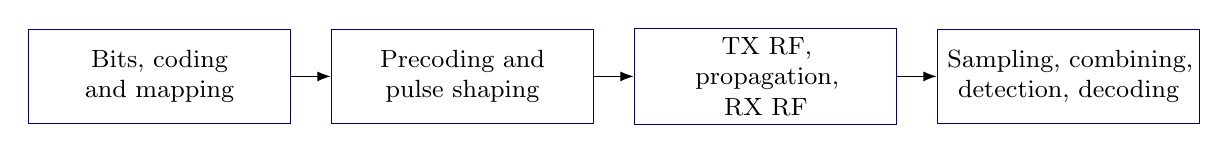
\begin{tikzpicture}[>=Latex,node distance=5mm,
b/.style={draw=blue!50!black,align=center,font=\small,text width=31mm,minimum height=12mm}]
\node[b] (a) {Bits, coding\\and mapping};
\node[b,right=of a] (b) {Precoding and\\pulse shaping};
\node[b,right=of b] (c) {TX RF,\\ propagation,\\RX RF};
\node[b,right=of c] (d) {Sampling, combining,\\detection, decoding};
\draw[->] (a)--(b);\draw[->] (b)--(c);\draw[->] (c)--(d);
\end{tikzpicture}
\caption{Conceptual signal flow. The effective digital channel represents the response between selected digital interfaces.}
\end{figure}

The physical antenna-to-antenna channel describes propagation and antenna interaction. The effective channel at the selected digital interfaces can additionally incorporate analog precoding or combining, RF responses, filtering, and sampling. The dimensions and interpretation of a channel matrix therefore depend on where its input and output interfaces are defined. The first part focuses on  the digital interfaces; later lectures distinguish antenna-, RF-chain-, and stream-level channels.

\subsection{Passband, baseband, and discrete time}
A real \ac{rf} waveform can be represented as
\begin{equation}\label{eq:rf}
s_{\mathsf{RF}}(t)=\sqrt2\,\RE{s(t)e^{j2\pi f_ct}},\qquad
s(t)=s_{\mathsf I}(t)+j s_{\mathsf Q}(t),\quad j^2=-1.
\end{equation}
The $\sqrt2$ convention makes carrier-averaged passband power equal complex-envelope power under the usual spectral-separation assumptions. Omitting it is also valid, but gives a different power normalization. Complex baseband retains amplitude and phase while removing the carrier oscillation. Two real I/Q components represent one complex envelope.
%
For instance, a coefficient $h=2e^{j\pi/3}$ scales amplitude by two and rotates phase by $\pi/3$, so its power gain is $\Abs{h}^2=4$. Symbol-time sampling after filtering generally produces a channel with memory:
\begin{equation}\label{eq:memory}
\ma{y}[n]=\sum_{\ell}\ma{H}[\ell]\ma{x}[n-\ell]+\ma{v}[n].
\end{equation}
The memoryless narrowband model requires approximately flat response, aligned timing, and negligible residual intersymbol interference. Sampling alone does not remove memory. Appendix~\ref{app:signals} explains the reduction.

\section{SISO, SIMO, MISO, and MIMO}
\subsection{Dimensions and conventions}
Let $\NT$ and $\NR$ denote the number of transmit and receive digital signal ports, defining the effective \ac{mimo} channel. Vectors are columns; channel rows index outputs and columns index inputs. $\mT{\ma{A}}$ is a transpose and $\mH{\ma{A}}$ a conjugate transpose. Physically, \ac{siso} links one transmit port to one receive port; \ac{simo} provides several observations of one transmitted signal; \ac{miso} permits multiple transmit contributions to one received signal; and \ac{mimo} provides multiple transmit signals and receive observations. The numbers of ports describe available interfaces, not automatically independent information streams.
\begin{center}
\begin{tabular}{llll}\toprule
Configuration & $\NT$ & $\NR$ & Model\\\midrule
SISO & 1 & 1 & $y=hx+v$\\
SIMO & 1 & $>1$ & $\ma{y}=\ma{h}x+\ma{v}$\\
MISO & $>1$ & 1 & $y=\mT{\ma{h}}\ma{x}+v$\\
MIMO & $>1$ & $>1$ & $\ma{y}=\ma{H}\ma{x}+\ma{v}$\\\bottomrule
\end{tabular}
\end{center}
In the \ac{miso} convention, $\ma{h}$ contains the channel coefficients directly. Some texts define a conjugated channel vector and use $\mH{\ma{h}}$ instead; these definitions cannot be exchanged without changing the phase weights. Receive combining is written $z=\mH{\ma{w}}\ma{y}$ and one-stream transmit precoding $\ma{x}=\ma{f}d$.

\subsection{The channel matrix as a spatial mixing operator}
The common model is
\begin{equation}\label{eq:mimo}
\boxed{\ma{y}=\ma{H}\ma{x}+\ma{v}},\quad
\ma{H}\in\compl^{\NR\times\NT},\quad
\ma{x}\in\compl^{\NT},\quad\ma{y},\ma{v}\in\compl^{\NR}.
\end{equation}
The coefficient $h_{ij}=\IndexM{\ma{H}}{i}{j}$ maps transmit port $j$ to receive port $i$. Entrywise,
\begin{equation}
y_i=\sum_{j=1}^{\NT}h_{ij}x_j+v_i.
\end{equation}
Equivalently, $\ma{H}\ma{x}=\sum_j\ma{h}_jx_j$ where $\ma{h}_j$ is channel column $j$. Each column is the receive-side spatial signature of one transmit-port signal: it describes the complex contributions of that input to all receive observations. When columns are linearly independent, their noiseless contributions can in principle be distinguished; when columns are dependent, some input combinations become indistinguishable. Their degree of separation and strengths also affect performance in noise.

\begin{example}{a complex two-port mixture}\label{ex:complex}
Let $\ma{H}=\begin{bmatrix}1&j\\1&-j\end{bmatrix}$, $\ma{x}=[1,j]^{\mathsf T}$, and $\ma{v}=\ma{0}$. Then $y_1=1+j^2=0$ and $y_2=1-j^2=2$.
Although the first observation vanishes due to destructive interference, no information is lost in the complete noiseless receive vector because the channel matrix is invertible. The two channel columns are orthogonal and $\mH{\ma{H}}\ma{H}=2\ma{I}_2$, so $\frac12\mH{\ma{H}}\ma{y}=\ma{x}$. In noise, this operation produces an estimate and also transforms the noise covariance.
\end{example}

\section{Rank, subspaces, and useful spatial dimensions}
\subsection{What rank reveals}
The range $\Range{\ma{H}}$ contains all possible noiseless outputs. Its dimension is $R_{\ma{H}}=\rank{\ma{H}}$, with
\begin{equation}\label{eq:rank}
R_{\ma{H}}\leq\min(\NT,\NR),\qquad \dim\Null{\ma{H}}=\NT-R_{\ma{H}}.
\end{equation}
If $\ma{u}$ belongs to the nullspace, $\ma{x}$ and $\ma{x}+\ma{u}$ produce the same noiseless observation. Full column rank is necessary for unique recovery of an arbitrary continuous input vector. Finite constellations can impose additional constraints; rank still counts the independent linear dimensions.

\begin{example}{same port count, different information}
Consider
\begin{equation}\label{eq:channels}
\ma{H}_1=\ma{I}_2,\qquad
\ma{H}_2=\begin{bmatrix}1&1\\1&1\end{bmatrix}.
\end{equation}
The first has rank two and returns the input vector. The second has rank one, and both outputs equal $x_1+x_2$. Its nullspace is $\Span{[1,-1]^{\mathsf T}}$. Inputs $[1,0]^{\mathsf T}$ and $[0,1]^{\mathsf T}$ therefore produce identical outputs. Repeating the same mixture can reduce noise but does not restore a missing dimension.

These examples isolate rank, not equal-gain performance: $\frob{\ma{H}_1}^2=2$ and $\frob{\ma{H}_2}^2=4$. For equal total squared gain, define $\widetilde{\ma{H}}_2=\ma{H}_2/\sqrt2$, so that $\frob{\widetilde{\ma{H}}_2}^2=2$ while its rank remains one. Equal Frobenius norm alone does not imply equal spectral efficiency or error performance.
\end{example}

\subsection{SVD: spatial directions and gains}
The \ac{svd} is
\begin{equation}\label{eq:svd}
\ma{H}=\ma{U}\ma{\Sigma}\mH{\ma{V}},
\end{equation}
where $\ma{U}$ and $\ma{V}$ are unitary and $\ma{\Sigma}$ is rectangular diagonal with nonnegative singular values. Let $R_{\ma{H}}=\rank{\ma{H}}$. There are $R_{\ma{H}}$ positive singular values $\sigma_1\geq\cdots\geq\sigma_s\geq\cdots\geq\sigma_{R_{\ma{H}}}>0$, indexed by $s=1,\ldots,R_{\ma{H}}$. Geometrically, SVD changes input coordinates, scales independent directions, and changes output coordinates. With $\ma{x}=\ma{V}\bar{\ma{x}}$ and $\bar{\ma{y}}=\mH{\ma{U}}\ma{y}$,
\begin{equation}
\bar{\ma{y}}=\ma{\Sigma}\bar{\ma{x}}+\bar{\ma{v}}.
\end{equation}
Transmit processing based on $\ma{V}$ requires transmitter \ac{csi}. Unitary receive processing preserves white-noise covariance; colored noise requires separate treatment. The decomposition is a way to understand the channel, even when a practical receiver uses another algorithm.

\begin{example}{full rank need not mean two strong streams}
For $\ma{H}_\epsilon=\diag{1,\epsilon}$ with $0<\epsilon\leq1$, rank is two but singular values are 1 and $\epsilon$. At $\epsilon=0.1$, inverting the second mode multiplies noise variance by 100. Its spectral condition number is $\Cond{\ma{H}_\epsilon}=1/\epsilon=10$. Whether the weak mode is useful depends on SNR and processing.
\end{example}
Three notions need to be distinguished: $\min(\NT,\NR)$ bounds the possible rank, $R_{\ma{H}}=\rank{\ma{H}}$ counts the nonzero independent channel modes, and $\NS$ denotes the number of streams selected for transmission. For independently recoverable linear streams, $\NS\leq R_{\ma{H}}$; at finite SNR it may be preferable to use fewer than $R_{\ma{H}}$ modes because small singular values correspond to weak channels and potentially strong noise enhancement. Later lectures explain how geometry, multipath, correlation, and hardware generate this structure.

\section{General narrowband digital processing}
\subsection{Assumptions and interfaces}
The course initially assumes a linear complex-baseband channel, negligible frequency selectivity and intersymbol interference, synchronized processing, an approximately constant channel over the block, digital access to the selected ports, and additive noise. Any example choosing processing from a known channel assumes the relevant \ac{csi}. These are modeling choices, not universal properties of wireless links.

\subsection{Streams, precoding, and combining}
Let $\ma{d}\in\compl^{\NS \times 1}$ contain the symbols of $\NS$ selected streams, not necessarily one stream per antenna. The precoder distributes those streams across the transmit ports; the combiner forms stream-level observations from the received ports. For the  digital interfaces,
\begin{align}
\ma{x}&=\ma{F}\ma{d},&\ma{F}&\in\compl^{\NT\times\NS},\\
\ma{y}_{\mathsf c}&=\mH{\ma{W}}\ma{y},&\ma{W}&\in\compl^{\NR\times\NS},\\
\ma{y}_{\mathsf c}&=\Hs\ma{d}+\ma{v}_{\mathsf c},&\Hs&=\mH{\ma{W}}\ma{H}\ma{F},\label{eq:stream}\\
\ma{v}_{\mathsf c}&=\mH{\ma{W}}\ma{v}.&&\nonumber
\end{align}
The stream-level matrix is $\NS\times\NS$ but need not be diagonal or invertible. Four ports can carry one stream or several. Independent linear stream recovery requires $\NS\leq\rank{\ma{H}}$ and processing that preserves those modes; this necessary condition does not guarantee reliable recovery in noise. The digital and analog frontend processing will be discussed in later lectures.

\begin{example}{dimensions before arithmetic}
For $\NT=4$, $\NR=3$, $\NS=2$, the channel is $3\times4$, precoder $4\times2$, and combiner $3\times2$. Thus $(2\times3)(3\times4)(4\times2)=2\times2$ for the effective channel. The Hermitian transpose on the combiner is essential.
\end{example}

\subsection{Second moments, power, and noise}
Define $\ma{R}_x=\Ex{\ma{x}\mH{\ma{x}}}$ and $\ma{R}_d=\Ex{\ma{d}\mH{\ma{d}}}$. These are second moments, equal to covariance for zero-mean vectors. In the discrete-time normalized channel model, squared signal amplitude measures transmit energy per channel use (often termed normalized transmit power). Thus,
\begin{equation}\label{eq:power}
P_x=\Ex{\NormTwo{\ma{x}}^2}=\trace{\ma{R}_x},\qquad
\ma{R}_x=\ma{F}\ma{R}_d\mH{\ma{F}}.
\end{equation}
With unit-energy pulses and symbol interval $T_{\mathsf s}$,
the trace represents the transmitted energy per symbol
interval. Here, one channel use corresponds to one symbol interval in the considered model. The corresponding average transmit power is
\begin{equation}
	\Ptx = \frac{P_x}{T_{\mathsf s}}.
\end{equation}
For normalized discrete-time models, energy per channel use
may be used as the power measure, provided that the adopted
normalization is explicitly stated. All comparisons must
consider the same total transmit-power budget.

For zero-mean noise, the covariance and
autocorrelation matrices coincide,
$\ma{C}_v=\ma{R}_v$. After linear combining,
the noise covariance becomes
\begin{equation}\label{eq:combinednoise}
	\ma{R}_{\widetilde v}
	=\mH{\ma{W}}\ma{R}_v\ma{W}.
\end{equation}
White noise has $\ma{R}_v=\sigma_v^2\ma{I}_{\NR}$. After combining its covariance is $\sigma_v^2\mH{\ma{W}}\ma{W}$. This is unchanged white noise for orthonormal combiner columns, but can be colored or unequally scaled otherwise.
The effective noise at the digital receive ports may already include the effects of analog and digital frontend processing. Consequently, even if noise introduced at an earlier receiver stage is spatially white, the effective noise need not be white.




For fixed $\ma{H}$ and zero-mean uncorrelated input and noise,
\begin{equation}
\ma{R}_y=\ma{H}\ma{R}_x\mH{\ma{H}}+\ma{R}_v.
\end{equation}
For a random channel, use conditional statistics given $\ma{H}$ and average over the channel when unconditional moments are wanted.

\begin{example}{fixed total budget}
With independent unit-variance streams and $\ma{F}=\sqrt{P_{x}/2}\ma{I}_2$, total transmitted power is $P_{x}$. Giving each port power $P_{x}$ instead doubles the total and confounds a spatial comparison with a power increase.
\end{example}

\subsection{Estimation and detection preview}
Channel estimation infers an unknown channel using known pilots. Data detection infers unknown symbols using channel knowledge. For white proper Gaussian noise and known $\ma{H}$, maximum-likelihood detection is
\begin{equation}\label{eq:ml}
\widehat{\ma{d}}_{\ML}=\argmin_{\ma{d}\in\set{D}^{\NS}}
\NormTwo{\ma{y}-\ma{H}\ma{F}\ma{d}}^2,
\end{equation}
where $\set{D}$ is a constellation. This finite search differs from unconstrained \ac{ls} followed by symbol slicing. \Ac{map} includes prior probabilities; \ac{mmse} minimizes mean-square error. Appendix~\ref{app:estimation} elaborates these distinctions.

\section{Course roadmap and recap}
Lecture~02 develops combining, precoding, SVD channels, capacity, and power allocation; Lecture~03 treats channel statistics and performance. Lectures~04--05 introduce multiuser, massive, and distributed MIMO, and Lecture~06 consolidates digital processing. Lectures~07--10 develop antenna geometry, beamforming, antenna responses, and physical channel construction. Lectures~11--13 extend to wideband, frequency-dependent processing, near-field, and XL-MIMO. Lecture~14 integrates the complete system and introduces sensing and localization.

The physical and effective channels will be distinguished more carefully when hybrid architectures are introduced. The notation follows the interface hierarchy
\begin{equation}
\underbrace{\Ha}_{\text{antenna elements}}
\ \longrightarrow\ 
\underbrace{\Hrf}_{\text{RF-chain interfaces}}
\ \longrightarrow\ 
\underbrace{\ma{H}}_{\text{selected digital interfaces}}
\ \longrightarrow\ 
\underbrace{\Hs}_{\text{data streams}}.
\end{equation}
Here $\ma{H}$ denotes the effective channel between the digital interfaces. The digital precoder $\ma{F}$ and combiner $\ma{W}$ map the data streams to the chosen channel input and output interfaces. Consequently, the stream-level relation retains the common form
\begin{equation}
\Hs=\mH{\ma{W}}\ma{H}\ma{F}.
\end{equation}
\paragraph{Exit questions.}
Can a $4\times4$ channel have only one useful mode? Can repeated receive observations improve SNR without increasing rank? Does every combiner preserve white noise? The answers are yes, yes, and no. Explain each using the model. Always specify interfaces, check dimensions, and fix power/noise conventions before comparing systems.

\clearpage\appendix
\section{Notation reference}\label{app:notation}
Scalars are italic, vectors/matrices bold lowercase/uppercase, sets calligraphic, and descriptive indices and transpose markers upright.
\begin{longtable}{p{0.29\linewidth}p{0.61\linewidth}}\toprule
Symbol & Meaning\\\midrule\endhead
$\compl,\real$ & Complex and real fields\\
$\mT{\ma{A}},\mH{\ma{A}},\mC{\ma{A}}$ & Transpose, Hermitian transpose, conjugation\\
$\NormTwo{\ma{x}},\frob{\ma{A}}$ & Euclidean and Frobenius norms\\
$\trace{\ma{A}},\rank{\ma{A}},\pinv{\ma{A}}$ & Trace, rank, pseudoinverse\\
$\NT,\NR,\NS$ & Transmit ports, receive ports, streams\\
$\ma{F},\ma{W}$& stream precoding/combining\\
$\Ha,\Hrf,\ma{H},\Hs$ & Antenna-element, RF-chain, selected digital-interface, and stream-level channels\\
$\ma{R}_x,\ma{C}_x$ & Second moment and centered covariance\\
$\sigma_v^2,\Nzero$ & Discrete noise variance and continuous PSD parameter\\
$\Ex{X},\CNormal$ & Expectation and proper complex Gaussian notation\\\bottomrule
\end{longtable}
One-based mathematical indexing is used by default, especially  for matrix indexing, unless using zero-based is explicitly stated. A covariance is centered unless zero mean is explicitly stated. Detailed notation for the complete course ia presented in the document \textit{00\_notation.pdf}. 

\section{Complex linear algebra}\label{app:algebra}
\subsection{Conjugation, inner products, and norms}
For $z=a+jb$, conjugation gives $\mC{z}=a-jb$ and $\Abs{z}^2=z\mC{z}=a^2+b^2$. Multiplication multiplies magnitudes and adds phases. For complex column vectors,
\begin{equation}
\inner{\ma{x}}{\ma{y}}=\mH{\ma{x}}\ma{y},\qquad
\NormTwo{\ma{x}}^2=\mH{\ma{x}}\ma{x}=\sum_i\Abs{x_i}^2.
\end{equation}
Conjugation is essential: $\ma{x}=[1,j]^{\mathsf T}$ has $\mT{\ma{x}}\ma{x}=0$, but $\mH{\ma{x}}\ma{x}=2$. Orthogonality means $\mH{\ma{x}}\ma{y}=0$. Cauchy--Schwarz states
\begin{equation}
\Abs{\mH{\ma{x}}\ma{y}}^2\leq\NormTwo{\ma{x}}^2\NormTwo{\ma{y}}^2.
\end{equation}
To prove it for nonzero $\ma{x}$, minimize $\NormTwo{\ma{y}-\alpha\ma{x}}^2\geq0$ over complex $\alpha$. Substitution of $\alpha=\mH{\ma{x}}\ma{y}/\NormTwo{\ma{x}}^2$ gives the inequality. Equality holds for linearly dependent vectors. This also explains why alignment with a channel maximizes a unit-norm   desired amplitude of the combiner.

Useful matrix identities are
\begin{equation}
\mH{(\ma{A}\ma{B})}=\mH{\ma{B}}\mH{\ma{A}},\qquad
\frob{\ma{A}}^2=\trace{\mH{\ma{A}}\ma{A}}=\sum_{i,j}\Abs{a_{ij}}^2.
\end{equation}
The trace is the sum of diagonal entries and is cyclic in conformable products: $\trace{\ma{A}\ma{B}}=\trace{\ma{B}\ma{A}}$. Cyclicity does not permit arbitrary reordering. The Frobenius norm measures total squared coefficient magnitude, not the number of independent modes.

\subsection{Bases, subspaces, and projections}
A span contains all linear combinations of specified vectors. A basis is an independent spanning set. If $\ma{Q}\in\compl^{N\times r}$ has orthonormal columns, $\mH{\ma{Q}}\ma{Q}=\ma{I}_r$, and
\begin{equation}
\ma{P}=\ma{Q}\mH{\ma{Q}},\qquad \mH{\ma{P}}=\ma{P},\qquad \ma{P}^2=\ma{P}
\end{equation}
projects onto its range. Every vector splits as $\ma{y}=\ma{P}\ma{y}+(\ma{I}-\ma{P})\ma{y}$, with orthogonal components. For full-column-rank $\ma{A}$, the same projection is $\ma{A}\inv{(\mH{\ma{A}}\ma{A})}\mH{\ma{A}}$. It separates the component consistent with the model from an orthogonal residual, providing the geometry of least squares.

\subsection{Hermitian EVD and positivity}
A Hermitian matrix satisfies $\ma{A}=\mH{\ma{A}}$ and admits
\begin{equation}\label{eq:evd}
\ma{A}=\ma{Q}\ma{\Lambda}\mH{\ma{Q}},\quad
\ma{\Lambda}=\diag{\lambda_1,\ldots,\lambda_N},
\end{equation}
with an orthonormal eigenbasis and real eigenvalues. It is positive semidefinite if $\mH{\ma{u}}\ma{A}\ma{u}\geq0$ for every vector, equivalently all eigenvalues are nonnegative. Positive definiteness requires strict positivity for nonzero vectors. Covariance and Gram matrices are positive semidefinite. A general square matrix need not have an orthonormal eigenbasis or even be diagonalizable, so the Hermitian EVD formula cannot be used without checking its assumptions.

\begin{example}{correlation eigenmodes}
For real $-1\leq\rho\leq1$, $\ma{C}=\begin{bmatrix}1&\rho\\\rho&1\end{bmatrix}$ has eigenvectors $[1,1]^{\mathsf T}/\sqrt2$ and $[1,-1]^{\mathsf T}/\sqrt2$, with eigenvalues $1+\rho$ and $1-\rho$. At $\rho=1$, the difference mode has zero variance. For complex correlation, conjugate off-diagonal entries give eigenvalues $1\pm\Abs{\rho}$.
\end{example}

\subsection{SVD and the Gram matrices}
For a rectangular channel, the full SVD uses $\ma{U}\in\compl^{\NR\times\NR}$, $\ma{V}\in\compl^{\NT\times\NT}$, and $\ma{\Sigma}\in\real^{\NR\times\NT}$. The compact rank-$R_{\ma{H}}$ form, with singular-mode index $s$, is
\begin{equation}
\ma{H}=\ma{U}_r\ma{\Sigma}_r\mH{\ma{V}_r}
=\sum_{s=1}^{R_{\ma{H}}}\sigma_s\ma{u}_s\mH{\ma{v}_s}.
\end{equation}
In particular,
\begin{align}
\mH{\ma{H}}\ma{H}&=\ma{V}\mH{\ma{\Sigma}}\ma{\Sigma}\mH{\ma{V}},\\
\ma{H}\mH{\ma{H}}&=\ma{U}\ma{\Sigma}\mH{\ma{\Sigma}}\mH{\ma{U}}.
\end{align}
The nonzero Gram eigenvalues are $\sigma_s^2$, for $s=1,\ldots,R_{\ma{H}}$. The first $R_{\ma{H}}$ left singular vectors span the range and the zero-gain right directions span the nullspace. The spectral norm is $\sigma_1$ and $\frob{\ma{H}}^2=\sum_{s=1}^{R_{\ma{H}}}\sigma_s^2$. For full column rank, spectral conditioning is $\sigma_1/\sigma_{\NT}$. Numerical rank needs a tolerance because a very small computed singular value may reflect finite precision.

\subsection{Pseudoinverse and least squares}
Every matrix has a Moore--Penrose pseudoinverse,
\begin{equation}
\pinv{\ma{H}}=\ma{V}_r\inv{\ma{\Sigma}_r}\mH{\ma{U}_r}.
\end{equation}
It reciprocates only positive singular values. $\widehat{\ma{x}}=\pinv{\ma{H}}\ma{y}$ minimizes $\NormTwo{\ma{y}-\ma{H}\ma{x}}^2$ and has minimum norm among the minimizers. For full column rank, normal equations yield
\begin{equation}
\mH{\ma{H}}(\ma{y}-\ma{H}\widehat{\ma{x}})=\ma{0},\qquad
\pinv{\ma{H}}=\inv{(\mH{\ma{H}}\ma{H})}\mH{\ma{H}}.
\end{equation}
For actual computation, QR or SVD is generally preferable to explicit Gram-matrix inversion, which squares the condition number.

For $\ma{H}_2$ in \eqref{eq:channels}, the pseudoinverse is $\frac14\begin{bmatrix}1&1\\1&1\end{bmatrix}$. With $\ma{y}=[2,2]^{\mathsf T}$, it returns $[1,1]^{\mathsf T}$, but every $[1+a,1-a]^{\mathsf T}$ produces that same output. The pseudoinverse cannot reconstruct an unobservable nullspace component.

For full-column-rank zero forcing in white noise, the error covariance is
\begin{equation}
\ma{C}_{\mathsf e}=\sigma_v^2\pinv{\ma{H}}\mH{(\pinv{\ma{H}})}
=\sigma_v^2\inv{(\mH{\ma{H}}\ma{H})}.
\end{equation}
Noise variance along singular mode $s$ is $\sigma_v^2/\sigma_s^2$, explaining weak-mode noise amplification.

\section{Probability and complex random vectors}\label{app:probability}
\subsection{Probability, expectation, and likelihood}
For discrete $X$, $\Ex{g(X)}=\sum_xg(x)p_X(x)$; for continuous $X$, $\Ex{g(X)}=\int g(x)f_X(x)\,dx$ when the expectation exists. A density is not a point probability. Conditional probabilities obey Bayes' rule, $p_{X|Y}(x|y)=p_{Y|X}(y|x)p_X(x)/p_Y(y)$ for $p_Y(y)>0$, with an analogous density expression. A likelihood holds the observation fixed and varies the candidate parameter; it is not automatically a distribution over that parameter.

\subsection{Complex variance, covariance, and second moments}
For $X=X_{\mathsf R}+jX_{\mathsf I}$ and $\mu_X=\Ex{X}$,
\begin{equation}
\Var{X}\define\Ex{\Abs{X-\mu_X}^2}
=\Var{X_{\mathsf R}}+\Var{X_{\mathsf I}}.
\end{equation}
For a vector,
\begin{align}
\ma{\mu}_x&=\Ex{\ma{x}},\\
\ma{C}_x&=\Ex{(\ma{x}-\ma{\mu}_x)\mH{(\ma{x}-\ma{\mu}_x)}},\\
\ma{R}_x&=\Ex{\ma{x}\mH{\ma{x}}}=\ma{C}_x+\ma{\mu}_x\mH{\ma{\mu}_x}.
\end{align}
The covariance entry is $\Ex{(x_i-\mu_i)\mC{(x_j-\mu_j)}}$. It is Hermitian positive semidefinite since
\begin{equation}
\mH{\ma{a}}\ma{C}_x\ma{a}=\Ex{\Abs{\mH{\ma{a}}(\ma{x}-\ma{\mu}_x)}^2}\geq0.
\end{equation}
Moreover $\Ex{\NormTwo{\ma{x}}^2}=\trace{\ma{C}_x}+\NormTwo{\ma{\mu}_x}^2$. For deterministic $\ma{A}$ and $\ma{y}=\ma{A}\ma{x}+\ma{b}$,
\begin{equation}\label{eq:covtrans}
\ma{\mu}_y=\ma{A}\ma{\mu}_x+\ma{b},\qquad
\ma{C}_y=\ma{A}\ma{C}_x\mH{\ma{A}}.
\end{equation}
The transformation need not be square or invertible. This identity is the basis of output-noise calculations.

\subsection{Properness, circular symmetry, and dependence}
Pseudocovariance is
\begin{equation}
\widetilde{\ma{C}}_x=\Ex{(\ma{x}-\ma{\mu}_x)\mT{(\ma{x}-\ma{\mu}_x)}}.
\end{equation}
A vector is proper if this vanishes. A proper scalar has equal real/imaginary variances and zero covariance between them. Circular symmetry means $e^{j\phi}\ma{x}$ has the same distribution for every common rotation $\phi$. With finite second moments, circular symmetry implies zero mean and properness. Properness alone does not imply circular symmetry: equiprobable \ac{qpsk} is proper but invariant only under discrete quarter-turns.

Uncorrelated variables need not be independent. For example, $X$ uniform on $[-1,1]$ and $Y=X^2$ are dependent, yet $\Ex{X}=\Ex{X^3}=0$ gives zero covariance. For jointly proper complex Gaussian vectors, zero cross-covariance does imply independence. In general complex models, ordinary covariance alone does not characterize all dependence.

\subsection{Proper complex Gaussian vectors}
The notation $X\sim\CNormal(\mu,\sigma^2)$ specifies independent Gaussian real/imaginary parts of $X-\mu$, each with variance $\sigma^2/2$. Its density and total complex variance are
\begin{equation}
f_X(x)=\frac{1}{\pi\sigma^2}e^{-\Abs{x-\mu}^2/\sigma^2},\qquad
\Ex{\Abs{X-\mu}^2}=\sigma^2.
\end{equation}
For a proper $N$-dimensional vector with positive-definite covariance,
\begin{equation}
f_{\ma{x}}(\ma{x})=
\frac{\exp\left[-\mH{(\ma{x}-\ma{\mu})}\inv{\ma{C}}(\ma{x}-\ma{\mu})\right]}
{\pi^N\Det{\ma{C}}}.
\end{equation}
For singular covariance, the distribution lies on a lower-dimensional affine subspace and this full-dimensional density is invalid. A nonzero-mean proper Gaussian is circular about its mean; the centered vector is invariant under rotations about zero.

White proper Gaussian noise is $\ma{v}\sim\CNormal(\ma{0},\sigma_v^2\ma{I})$. Components are independent, with total complex variance $\sigma_v^2$ each. It can be generated as
\begin{equation}
\ma{v}=\frac{\sigma_v}{\sqrt2}(\ma{g}_{\mathsf R}+j\ma{g}_{\mathsf I}),
\end{equation}
using independent unit-variance real Gaussian vectors. Deterministic linear transforms preserve Gaussianity and properness, with covariance \eqref{eq:covtrans}. For a zero-mean scalar, magnitude is Rayleigh with density $2r e^{-r^2/\sigma^2}/\sigma^2$, $r\geq0$, and phase is independent uniform on $[0,2\pi)$.

\subsection{Whitening}
If $\ma{C}=\ma{Q}\ma{\Lambda}\mH{\ma{Q}}$ is positive definite, define $\ma{C}^{-1/2}=\ma{Q}\diag{\lambda_1^{-1/2},\ldots,\lambda_N^{-1/2}}\mH{\ma{Q}}$. Then $\ma{C}^{-1/2}(\ma{x}-\ma{\mu})$ has identity covariance. Whitening noise in a MIMO model replaces the channel by $\ma{R}_v^{-1/2}\ma{H}$. Distances become $\mH{\ma{e}}\inv{\ma{R}_v}\ma{e}$. Singular covariance requires restriction to its supported subspace.

\section{Estimation and detection}\label{app:estimation}
\subsection{Pilot-based channel estimation}
Collect $T$ known transmit vectors in $\ma{X}\in\compl^{\NT\times T}$ and receive vectors in $\ma{Y}\in\compl^{\NR\times T}$. For a constant channel,
\begin{equation}
\ma{Y}=\ma{H}\ma{X}+\ma{V},\qquad
\widehat{\ma{H}}_{\LS}=\ma{Y}\pinv{\ma{X}}.
\end{equation}
This is the minimum-Frobenius-norm least-squares solution. Unique identification of an arbitrary channel needs $\rank{\ma{X}}=\NT$ and hence $T\geq\NT$. With full row rank,
\begin{equation}
\widehat{\ma{H}}_{\LS}=\ma{Y}\mH{\ma{X}}\inv{(\ma{X}\mH{\ma{X}})}.
\end{equation}
For orthogonal pilots $\ma{X}\mH{\ma{X}}=E_{\mathsf p}\ma{I}$ and independent white noise entries of variance $\sigma_v^2$, each channel coefficient has estimation-error variance $\sigma_v^2/E_{\mathsf p}$.

\begin{example}{two pilots reveal two columns}
With $\ma{X}=\sqrt{E_{\mathsf p}}\ma{I}_2$ and no noise, the two receive vectors are the two channel columns scaled by $\sqrt{E_{\mathsf p}}$. Repeating only $[1,1]^{\mathsf T}$ instead reveals their sum and cannot distinguish the columns.
\end{example}

\subsection{ML, MAP, MMSE, and LMMSE}
Let $\ma{G}=\ma{H}\ma{F}$ and $\ma{e}(\ma{d})=\ma{y}-\ma{G}\ma{d}$. With positive-definite proper Gaussian noise covariance, ML minimizes $\mH{\ma{e}}\inv{\ma{R}_v}\ma{e}$. For discrete candidates, MAP adds a prior:
\begin{equation}
\widehat{\ma{d}}_{\MAP}=\argmin_{\ma{d}\in\set{D}^{\NS}}
\left[\mH{\ma{e}(\ma{d})}\inv{\ma{R}_v}\ma{e}(\ma{d})-\ln p_{\ma{d}}(\ma{d})\right].
\end{equation}
Equal priors give identical \ac{ml} and \ac{map} decisions. Finite-constellation search is different from unconstrained least squares followed by slicing.

The unconstrained \ac{mmse} estimate is $\Ex{\ma{d}\mid\ma{y}}$. To see its optimality, write $\ma{m}(\ma{y})=\Ex{\ma{d}\mid\ma{y}}$ and use conditional orthogonality:
\begin{equation}
\Ex{\NormTwo{\ma{d}-\ma{g}(\ma{y})}^2}
=\Ex{\NormTwo{\ma{d}-\ma{m}(\ma{y})}^2}
+\Ex{\NormTwo{\ma{m}(\ma{y})-\ma{g}(\ma{y})}^2}.
\end{equation}
The second term is nonnegative. A posterior mean can lie between constellation points; minimizing \ac{mse} differs from minimizing symbol error probability.

For zero-mean data  uncorrelated with noise, the best complex-linear estimator is
\begin{equation}
\widehat{\ma{d}}_{\LMMSE}=\ma{R}_d\mH{\ma{G}}
\inv{(\ma{G}\ma{R}_d\mH{\ma{G}}+\ma{R}_v)}\ma{y},
\end{equation}
when the inverted covariance is positive definite. The orthogonality equation $\Ex{(\ma{d}-\ma{A}\ma{y})\mH{\ma{y}}}=\ma{0}$ derives this result. Gaussianity is not required for optimality within the linear class. For jointly proper Gaussian variables LMMSE equals MMSE; improper models may benefit from also using $\mC{\ma{y}}$.

\begin{example}{regularizing a weak mode}
For $y=hd+v$, the LMMSE coefficient is $P_d\mC{h}/(P_d\Abs{h}^2+\sigma_v^2)$. With $h=0.1$, $P_d=1$, and $\sigma_v^2=0.1$, it is approximately 0.909; zero forcing uses 10. LMMSE accepts bias to avoid excessive noise amplification.
\end{example}

\section{Information-theoretic reference}
For a fixed channel, proper Gaussian input and independent white Gaussian noise give mutual information per complex use
\begin{equation}
I(\ma{x};\ma{y}\mid\ma{H})=\log_2\Det{\ma{I}_{\NR}+\frac{1}{\sigma_v^2}\ma{H}\ma{R}_x\mH{\ma{H}}}.
\end{equation}
Capacity maximizes this over positive-semidefinite $\ma{R}_x$
subject to a total transmit-energy budget $\Ed$ per channel use,
$\trace{\ma{R}_x}\leq E_d$, under the specified
channel-knowledge assumptions.

With equal power allocation across the $\NT$ transmit
dimensions and full utilization of the budget,
\begin{equation}
	I=\sum_{s=1}^{R_{\ma{H}}}
	\log_2\left(
	1+\frac{\Ed\sigma_s^2}{\NT\sigma_v^2}
	\right).
\end{equation}
Equal allocation is not generally optimal when transmitter CSI permits adaptation. At high SNR, fixed-channel rate grows as $R_{\ma{H}}\log_2(\Ed/\sigma_v^2)$ plus a channel-dependent constant, assuming fixed channel coefficients and a full-rank power allocation over all nonzero modes. Rank sets this slope; singular values determine finite-SNR usefulness. Water-filling, fading averages, and outage are developed in Lectures~02--03.

\clearpage
\section{Signal-model reference}\label{app:signals}
Expanding \eqref{eq:rf} gives $s_{\mathsf{RF}}(t)=\sqrt2[s_{\mathsf I}(t)\cos(2\pi f_ct)-s_{\mathsf Q}(t)\sin(2\pi f_ct)]$. Ideal quadrature downconversion and low-pass filtering recover the envelope with matching oscillator and gain conventions. Carrier mismatch adds a time-dependent phase; synchronization is necessary for the simple model.

For a unit-energy pulse $p(t)$ and symbol interval $T_{\mathsf s}$, transmit envelope $s_j(t)=\sum_nx_j[n]p(t-nT_{\mathsf s})$. A baseband response $c_{ij}(t)$ followed by matched filtering produces taps
\begin{equation}
g_{ij}[\ell]=\left.(p*c_{ij}*p^*(-\cdot))(t)\right|_{t=\ell T_{\mathsf s}},
\end{equation}
where $*$ denotes convolution and $p^*(-\cdot)$ the matched filter. Therefore $y_i[n]=\sum_j\sum_\ell g_{ij}[\ell]x_j[n-\ell]+v_i[n]$. If $c_{ij}(t)\approx h_{ij}\delta(t)$ after timing alignment and pulse autocorrelation is Nyquist at symbol samples, only $g_{ij}[0]\approx h_{ij}$ remains.

A rule of thumb for flat fading is occupied bandwidth times relevant delay spread much smaller than one. Block duration should be short relative to coherence time. Filtered noise need not be temporally white without suitable pulse/noise assumptions. Wideband channels retain multiple taps; later OFDM processing produces approximately narrowband subcarrier models under cyclic-prefix and synchronization conditions.

\clearpage
\section{Introductory tutorial and answers}
All unspecified noise terms are zero. Exercises E1--E6 cover the main introductory lecture; E7--E12 extend to noise, inversion, estimation, and rate and can be assigned as preparation for later lectures. Complete the exercises before checking the answers.
\begin{enumerate}[label=\textbf{E\arabic*.}]
\item Identify the configuration and maximum rank for $(\NT,\NR)=(1,4),(4,1),(3,2),(1,1)$.
\item For $\ma{a}=[1,j]^{\mathsf T}$ and $\ma{b}=[j,1]^{\mathsf T}$, find $\mT{\ma{a}}\ma{b}$, $\mH{\ma{a}}\ma{b}$, and $\NormTwo{\ma{a}}^2$. Are they orthogonal?
\item Use the channel of Example~\ref{ex:complex} with input $[1,-j]^{\mathsf T}$. Find its output and recover the input.
\item Find the ranks and nullspaces of \eqref{eq:channels}. Exhibit indistinguishable inputs for the second channel.
\item For $(\NT,\NR,\NS)=(4,3,2)$, give dimensions of $\ma{F}$, $\ma{W}$, $\Hs$, $\ma{R}_x$, and $\ma{R}_{\widetilde v}$. Is rank two guaranteed?
\item If $\ma{R}_d=\ma{I}_2$ and $\ma{F}=\sqrt3\ma{I}_2$, find total power. Rescale for total power 3.
\item Compare combined-noise covariance for $\ma{W}=\ma{I}_2$ and $\ma{W}=\diag{1,2}$ with input noise variance $\sigma_v^2$.
\item For $\ma{H}=\diag{1,0.1}$ and $\sigma_v^2=0.01$, find singular values, condition number, and ZF error covariance.
\item For $\ma{H}_2$ and output $[2,2]^{\mathsf T}$, find the pseudoinverse solution and explain the ambiguity.
\item A proper Gaussian scalar has complex variance 4. What are its real/imaginary variances? Is equiprobable QPSK circular under every rotation?
\item With pilots $\ma{X}=2\ma{I}_2$ and $\ma{Y}=\begin{bmatrix}2&2j\\2&-2j\end{bmatrix}$, estimate the channel. Would one pilot identify an arbitrary two-port channel?
\item Compare equal-allocation rate for the identity two-port channel, total power 10, and noise variance 1 with SISO using the same budget.
\end{enumerate}
\clearpage
\subsection*{Answers}
\begin{enumerate}[label=\textbf{E\arabic*.}]
\item SIMO, MISO, MIMO, SISO; maximum ranks 1, 1, 2, 1.
\item $2j$, 0, 2. The Hermitian inner product vanishes, so they are orthogonal.
\item Output $[2,0]^{\mathsf T}$; $\frac12\mH{\ma{H}}$ returns $[1,-j]^{\mathsf T}$.
\item Ranks 2 and 1; nullspaces $\{\ma{0}\}$ and $\Span{[1,-1]^{\mathsf T}}$. Inputs $[1,0]^{\mathsf T}$ and $[0,1]^{\mathsf T}$ give the same output for the second.
\item $4\times2$, $3\times2$, $2\times2$, $4\times4$, $2\times2$. Rank two is not guaranteed; channel or processing can remove a mode.
\item Total power 6. Use $\sqrt{3/2}\ma{I}_2$ for power 3.
\item $\sigma_v^2\ma{I}_2$ versus $\sigma_v^2\diag{1,4}$.
\item Singular values 1 and 0.1; condition number 10; error covariance $\diag{0.01,1}$.
\item Minimum-norm solution $[1,1]^{\mathsf T}$. A nullspace component is unobservable.
\item Real/imaginary variances are 2 each. QPSK is proper but not invariant under arbitrary rotations.
\item $\widehat{\ma{H}}=\ma{Y}/2$. A single pilot has rank at most one and cannot identify two arbitrary channel columns.
\item $2\log_2(6)\approx5.170$ bit/use versus $\log_2(11)\approx3.459$ bit/use.
\end{enumerate}

\section*{Reading and source notes}
Further reading: D. Tse and P. Viswanath, \emph{Fundamentals of Wireless Communication}, Cambridge University Press, 2005. Chapters 2--3 cover channels and diversity; Chapters 7--8 cover MIMO; Appendix A covers Gaussian detection and estimation.\\ Author-provided chapters: \url{https://web.stanford.edu/~dntse/wireless_book.html}.

\end{document}

